\section{Konseptutvikling}
\label{sec:konseptutvikling}
Hovedfunksjonen er å omforme energien fra ett opptrekk til fremdrift. Delfunksjonene er å tilføre energi, lagre energi i svinghjulet, overføre bevegelse til drivhjulene, bære og rette opp komponentene og sikre kontakt med underlaget.

Det er utviklet tre konsepter for overføringen fra svinghjul til drivhjul, vist i figur~\ref{fig:konsepter}. Alle bruker det utdelte svinghjulet, opptrekk med snor via en trommel på svinghjulsakselen og en ramme av to sideplater. Konseptene skiller seg i hvordan utvekslingen $i = \omega_s/\omega_h$ mellom svinghjul og drivhjul er løst.

\begin{figure}[htbp]
    \centering
    \begin{subfigure}[b]{0.48\textwidth}
        \centering
        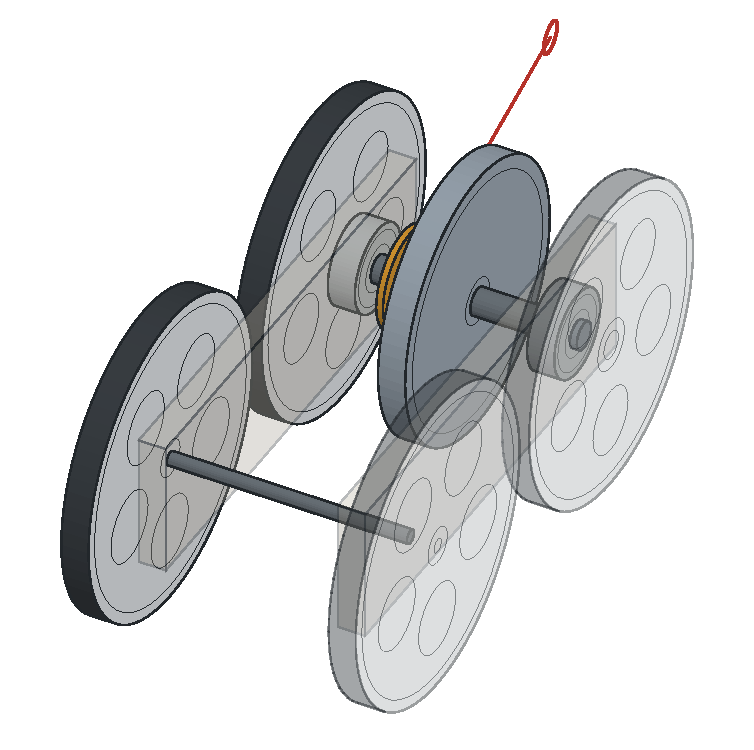
\includegraphics[width=\textwidth]{Images/Konsepter/konsept1_direkte.pdf}
        \caption{Konsept 1: direkte drift, $i = 1$.}
        \label{fig:konsept1}
    \end{subfigure}
    \hfill
    \begin{subfigure}[b]{0.48\textwidth}
        \centering
        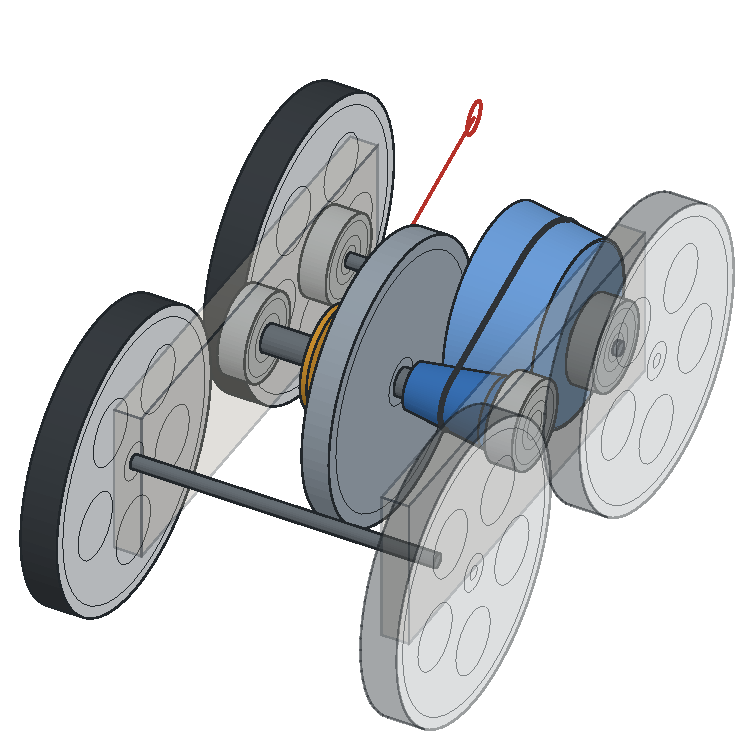
\includegraphics[width=\textwidth]{Images/Konsepter/konsept2_cvt.pdf}
        \caption{Konsept 2: kjegle-CVT, $i \approx 2{,}6$--$4{,}4$.}
        \label{fig:konsept2}
    \end{subfigure}

    \vspace{2ex}
    \begin{subfigure}[b]{0.48\textwidth}
        \centering
        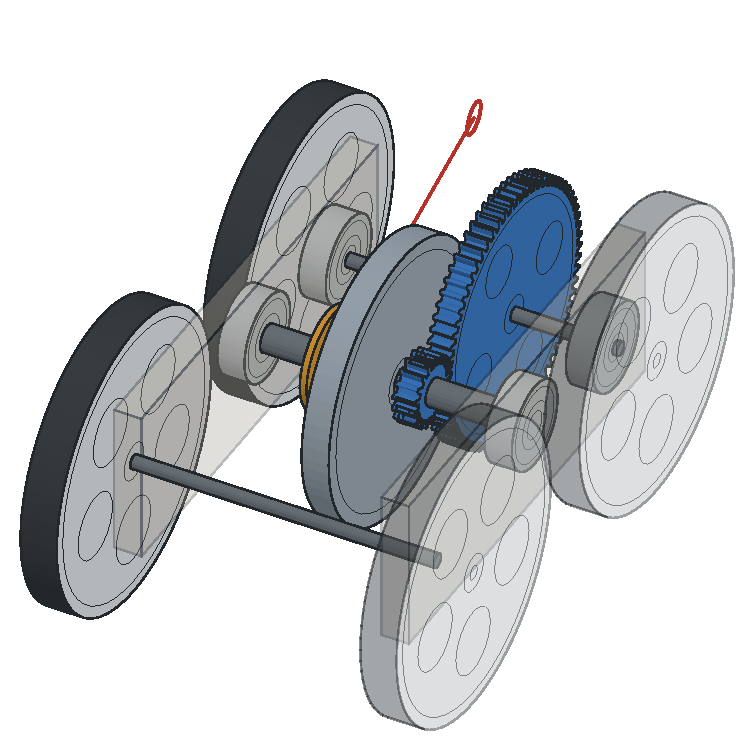
\includegraphics[width=\textwidth]{Images/Konsepter/konsept3_tannhjul.pdf}
        \caption{Konsept 3: tannhjul 17\,:\,68, $i = 4$.}
        \label{fig:konsept3}
    \end{subfigure}
    \caption{Konseptskisser av drivverket, sett fra venstre side, foran og ovenfra. Hjulene nærmest betrakteren er vist gjennomsiktige. Utvekslingen er blå, snortrommelen oransje og snora rød.}
    \label{fig:konsepter}
\end{figure}

\subsection{Konsept 1: Direkte drift}
Svinghjulet sitter på drivakselen, slik at $i = 1$ (figur~\ref{fig:konsept1}). Konseptet har færrest deler, men drivhjulene må ha større diameter enn svinghjulet, her \SI{68}{mm}, for at svinghjulet skal gå klar av underlaget. Uten nedgiring blir farten svært høy, i teorien omtrent \SI{14}{m/s} ved \SI{4000}{o/min}, og en stor del av energien går tapt som slur mellom hjul og underlag når bilen settes ned.

\subsection{Konsept 2: Trinnløs utveksling (CVT)}
To motsatt vendte kjegler sitter på svinghjulsakselen og drivakselen, med en O-ring som reim mellom dem (figur~\ref{fig:konsept2}). Kjeglen på svinghjulsakselen går fra \SI{10}{mm} til \SI{15}{mm} i diameter, og kjeglen på drivakselen fra \SI{44}{mm} til \SI{39}{mm}. Når reimen flyttes langs kjeglene, endres utvekslingen trinnløst fra omtrent 4,4 til 2,6. Den beste utvekslingen kan dermed finnes ved testing uten å bytte deler, men reimen kan slure, og friksjonstapene blir større enn i et tannhjulsinngrep. Konseptet har også flest deler som må tilpasses.

\subsection{Konsept 3: Fast tannhjulsutveksling}
Et pinjong med 17 tenner på svinghjulsakselen driver et tannhjul med 68 tenner på drivakselen, med modul 0,8 (figur~\ref{fig:konsept3}). Det gir $i = 4$. Drivhjulene har diameter \SI{64}{mm}, og svinghjulsakselen og drivakselen er lagret i fire kulelagre av typen 626. Tannhjulsinngrepet overfører momentet uten slur og med lite tap. Utvekslingen er fast, men flere tannhjulspar med samme akseavstand kan prøves uten å endre rammen.

\begin{comment}
\subsection{Konseptevaluering}
Konseptene vurderes først mot obligatoriske krav og deretter mot forventet kjøredistanse, friksjon, driftssikkerhet, produserbarhet og justerbarhet. Vekter og vurderinger begrunnes før sluttkonsept velges.
% Sett inn vurderingsmatrise som tabell, med vekter og poeng per konsept, og begrunn valgt konsept.
% Beskriv hvilke antakelser som skal undersøkes gjennom prototyping.
\end{comment}
